\documentclass{beamer}

%gets rid of bottom navigation bars
\setbeamertemplate{footline}[page number]{}

%gets rid of navigation symbols
\setbeamertemplate{navigation symbols}{}

\title{Single-cell RNA sequencing for beginners}

\author{Aaron Lun \\[0.1in]
\footnotesize{CRUK Cambridge Institute}
}

\date{
\footnotesize{Tel Aviv University}\\[0.1in]
23 May 2018
}


\makeatletter
\newlength\beamerleftmargin
\setlength\beamerleftmargin{\Gm@lmargin}
\makeatother

\begin{document}
\maketitle

\begin{frame}{Why do single-cell RNA sequencing?}

\begin{exampleblock}{Why single cells?}
A lot of biology occurs at the cellular level:
\begin{itemize}
\item Cell identity (e.g., cell types)
\item Cell behaviour and status (e.g., stress, metabolism, cell cycle)
\item Cellular dynamics (differentiation, activation)
\end{itemize}
\end{exampleblock}

\begin{exampleblock}{Why RNA sequencing?}
Quantify expression of every gene\footnote{poly A'd} in the transcriptome:
\begin{itemize}
\item FACS: small number of proteins
\item FISH: small number of transcripts
\end{itemize}
\end{exampleblock}
\end{frame}

\begin{frame}{A ``typical'' scRNA-seq protocol}
\noindent\makebox[\textwidth]{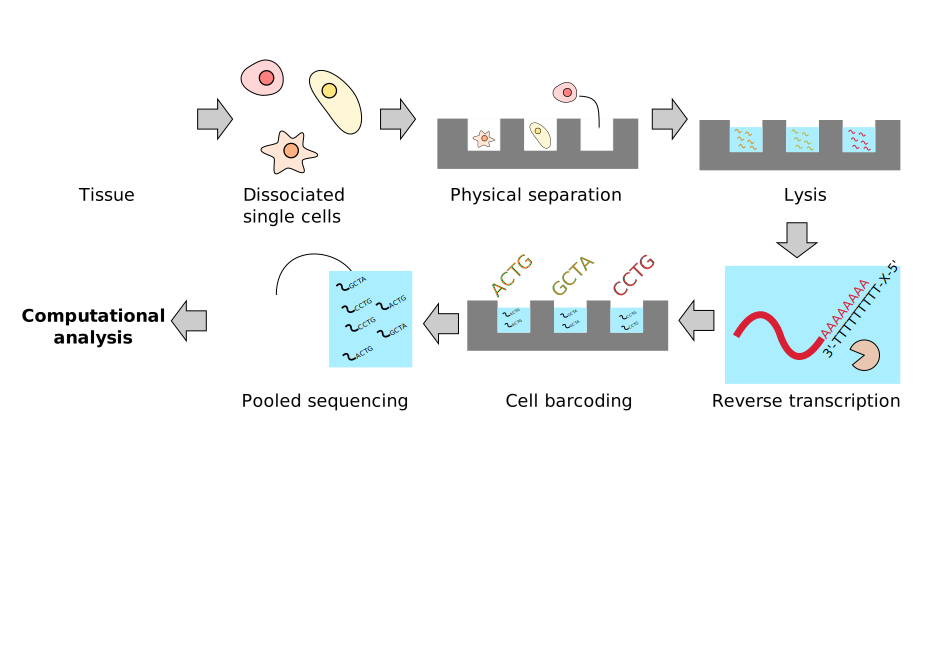
\includegraphics[width=0.95\paperwidth]{pics/overview.pdf}}\\[0.1in]

\begin{itemize}
\item Dissociation can be easy (blood) or hard (tumours).
\item Protocols differ in how they perform separation and RT.
\end{itemize}
\end{frame}

\begin{frame}{Physical separation methods: microfluidics}
Most popular of which is the Fluidigm C1:
\begin{center}
\includegraphics[width=0.7\textwidth]{pics/fluidigm_c1.jpg}
\end{center}
Less common nowadays due to cost, throughput, doublet issues
\end{frame}

\begin{frame}{Physical separation methods: cell sorting}
Sort individual cells into 96/384-well plates (``plate-based''):

\begin{center}
\includegraphics[width=0.5\textwidth]{pics/facs_to_plate.pdf}
\end{center}

Cheap, provides extra phenotypic data, easy to customize.
\end{frame}

\begin{frame}{Physical separation methods: droplets}
Capture cells in droplets in a water-in-oil emulsion:

\begin{center}
\includegraphics[width=0.65\textwidth]{pics/droplets.pdf}
\end{center}

High throughput (4000-10000 per run), lower coverage, noisier. 
\end{frame}







\end{document}
